\label{sec:H2PrevSum}
Our purpose here is to provide a summary of the major features of $\htwo$ preview controllers, which will hopefully be of assistance to control system designers. While some of these results are known within the control systems community, they are spread over many publications spanning three decades. 
\subsection{Generic Controller features} \label{generic:features}
\begin{description}
\item[Riccati Equation Solutions.] Synthesizing the output-feedback controller requires the solution of a full-information Riccati equation and a Kalman filtering equation \cite{LimebeerGreen,ZDG}. Although these equations appear to be of high order, the full-information control problem only requires the solution of the $n_g$-dimensional Ricatti equation (\ref{eqn:Xgg}), while the estimation problem requires the solution of the $n_g$-dimensional Riccati equation (\ref{eqn:Y2g}). The bulk of the full-information Riccati equation can be evaluated using the linear equations (\ref{eqn:Xgd}) and (\ref{eqn:Xdd}). The DARE (\ref{eqn:Xgg}) is precisely that which would be obtained if one were to search for a full information controller which minimised $\nrm{T_{w\rightarrow z}}$.

It is important to note that $F_{2g}$ and $\bar R$ are not functions of $X_{gd}$ or $X_{dd}$, and so (\ref{eqn:Xgg}) may be solved independently of (\ref{eqn:Xgd}) and (\ref{eqn:Xdd}). However, (\ref{eqn:Xgd}) depends on the solution of (\ref{eqn:Xgg}), and (\ref{eqn:Xdd}) depends on both (\ref{eqn:Xgg}) and (\ref{eqn:Xgd}). Lemma~\ref{lem:SylvRecurs} provides a fast algorithm for solving (\ref{eqn:Xgd}).
\item[Full-information control structure.] The full-information control signal has the form
\als{
u(k)^*=\hat u(k)+\sum_{j=0}^{N-1}{F_{2p,j}r(k-N+j)},
}
in which $\hat u(k)$ is a linear function of the states of $G$ and $W_r$, and of the signals $\eta$ and $w$; the $F_{2p,j}$'s are sometimes referred to as the `preview gains'. Further insight into the structure and role of the control signal components can be found in Remarks~\ref{rem:PrevGainInterp}, \ref{rem:SmallPrevGain} and \ref{rem:FIminwandr}.
\item[The preview gains decay to zero as $N \rightarrow \infty$.] It was first noted in \cite{Tomizuka_1975_OptDiscretePreview} that the magnitude of the preview gains approaches zero as $N$ approaches infinity; this follows from equation (\ref{eqn:F2pEff}) and $\lim_{N \rightarrow \infty} A^N_{cg} = 0$. As a consequence, far-distant preview information is relatively less important and the optimal infinite preview controller can be approximated  to arbitrary accuracy using a finite preview length.
\item[The controller has FIR (preview) and IIR components.]
Discrete-time preview controllers are composed of a high-order Finite Impulse Response (FIR) preview component, and low-order Infinite Impulse Response (IIR) components. This structure is illustrated in Figure~\ref{fig:PrevContStruct}, and is also highlighted in the continuous-time case in \cite{Moelja_2006_H2PreviewMultiple}. A proof is provided for the discrete-time case in Section \ref{sec:H2OF}. If the controller is written in observer form, then the states of the FIR preview block and the order $n_r$ IIR block are (perfect) reconstructions of the states of $\Phi$ and $W_r$ respectively. The state of the order $n_g$ IIR block is an estimate for the state of $G$.
\item[The controller is essentially low-order.] 
A discrete-time FIR transfer function can be realised using a shift-register to update the state, and a gain array to compute the output. This representation leads to the low-order controller representation in Figure~\ref{fig:PrevContStructxp}, where $\bar{K}$ is given by (\ref{low_order_K}). 
{
\stdcontrolfrags
\psfrag{Kbar}{$\bar K$}
\psfrag{Kr}{$K_r$}
\psfrag{r}{$r(k)$}
\psfrag{y}{$y(k)$}
\psfrag{u}{$u(k)$}
\psfrag{xp}{$\ma{r(k-N)\\\vdots\\r(k-1)}$}
\begin{figure}
\begin{center}
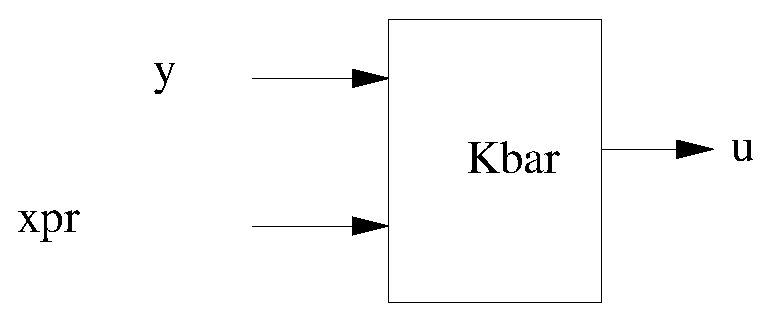
\includegraphics[width=0.5\columnwidth]{./diags/PrevContStructxpKbar.eps}
\caption{\label{fig:PrevContStructxp} The structure of the $\htwo$-optimal discrete-time preview controller. The signal $u(k)$ is the control, the measurement is $y(k)$, and $r(k)$ is the future-most value of the previewable disturbance.}
\end{center}
\end{figure}}
\item[The optimal control is independent of $W_r$ for large $N$]
This phenomenon was first noticed in \cite{Tomizuka_1975_OptDiscretePreview}, with a proof provided in Section \ref{sec:H2FI}. It is instructive to consider the influence of $W_r$ from a stochastic perspective. Since $\eta$ is assumed to be a realisation of a white-noise process, then a dynamic $W_r$ provides statistical information on future values of $r$. If, for example, $W_r$ is low-pass, the $r(k)$'s will become correlated and hence $W_r$ will introduce `statistical preview' beyond the preview horizon. We would therefore expect $W_r$ to reduce the need for preview, and also that its influence on the control would decline as $N$ tends to infinity.
\item[The optimal $\nrm{T_{w\rightarrow z}}_2$ is independent of $W_r$.]
In contrast with the $\hinf$ case \cite{Hazell_2007_DiscreteHinfPreview}, there is no conflict between the rejection of $w$ and the rejection of $\eta$; a proof of this is provided in Section \ref{sec:H2OF}.
\item[Noisy preview signals require a high-order controller.]
One might consider an uncertain preview problem, where the controller has access only to a noise-corrupted version of the previewed signal. 
In this scenario, the states of $\Phi$ are not known, and must be estimated. The preview provides benefit both by reducing the Full Information control cost, and by reducing the estimation cost. Estimating the states of $\Phi$ is a type of fixed-lag smoothing problem. Low-order implementations of fixed-lag smoothers are given in \cite{Anderson_1979_OptimalFiltering}, but these implementations are not usable here, because of the need for an estimate of all of the states of $\Phi$, rather than just the output of $\Phi$. The resulting controller is thus of the same order as the augmented plant. A controller for this problem may be synthesised by direct application of the results in Section \ref{subsec:stdH2OF}.
\end{description}
\subsection{Design Insights}
This section provides a number of `rules of thumb' that the authors have found useful. For the purposes of illustration, we will consider the full-information preview tracking problem described in Figure~\ref{fig:PrevTrackSysFI}, where $G$ is given by:
\begin{eqnarray}
\hat G&=&\frac{1.26 \times 10^{-8} (\z+1)^3}{
		(\z-1) (\z^2  - 1.998\z + 0.998)} \nonumber \\
G&=&\ma{\hat G\\1}. \label{example}
\end{eqnarray}
\begin{figure}
\begin{center}
\psfrag{W_e}{$W_e$}
\psfrag{z1}{$z_1$}
\psfrag{z2}{$z_2$}
\psfrag{W_r}{$W_r$}
\psfrag{u}{$u$}
\psfrag{r}{$r$}
\psfrag{G}{$G$}
\psfrag{zg}{$z_g$}
\psfrag{Phi}{$\Phi$}
\psfrag{W_r}{$W_r$}
\psfrag{eta}{$\eta$}
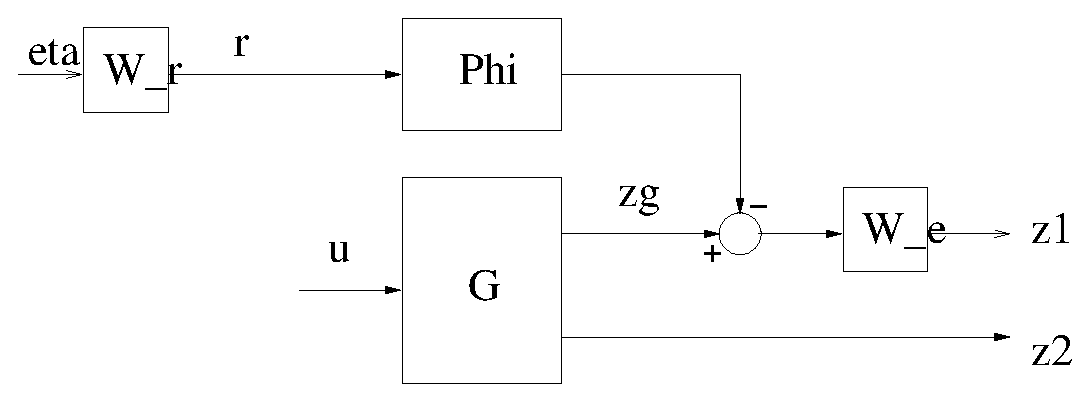
\includegraphics[width=0.75\columnwidth]{./diags/PrevTrackSysFI.eps}
\end{center}
\caption{A simple preview tracking problem. The feedback signal is derived from the states of $G$, $W_r$, $W_e$ and $\Phi$, together with $\eta$. The signal $u$ is the control, $r$ is the previewed reference, and $z=\left[z_1'\,\,z_2'\right]'$ is the output to be minimized. \label{fig:PrevTrackSysFI}}
\end{figure}
The discrete transfer function $\hat G$ was obtained by discretising
\als{       \frac{101}{s (s^2 + 2s + 101)},}
using a sample time of 0.001 seconds.
We search for a $K$ which minimises $\nrm{T_{\eta\rightarrow z}}_{2,\infty}$, or equivalently, the $K$ which minimises:
\aln{
\nrm{\ma{W_eW_rT_{r\rightarrow e}\\W_rT_{r\rightarrow u}}}_{2,\infty} \label{eqn:DesInsightCL}
.}
Clearly this represents a tracking problem in which minimisation of tracking errors must be balanced against  excessive control requirements. The transfer functions $W_r$ and $W_e$ may be chosen to reflect, respectively, the expected frequency content of $r$, and the importance of achieving good tracking at a given frequency. We will now use this example to illustrate some general properties of $\htwo$ preview tracking controllers.

\begin{description}
\item[Preview improves steady-state disturbance rejection.] 
Figure~\ref{fig:BetterSSWithIncN} illustrates the `non-responsiveness' of the closed-loop system in the case of no reference weight, and a low preview horizon. In the limiting case, where there is zero preview and no reference weighting, the controller does not have any information about the value of the reference at the next time step, and so it cannot make a decision about the direction in which to send the plant. Therefore, the tracking error cost cannot be reduced, and so the optimal controller can only minimise the control cost, leading to a choice of $u=0$.

Alternatively, as $N\rightarrow \infty$, then the steady state error tends towards zero (in the absence of disturbances or modelling errors). 
\begin{figure}
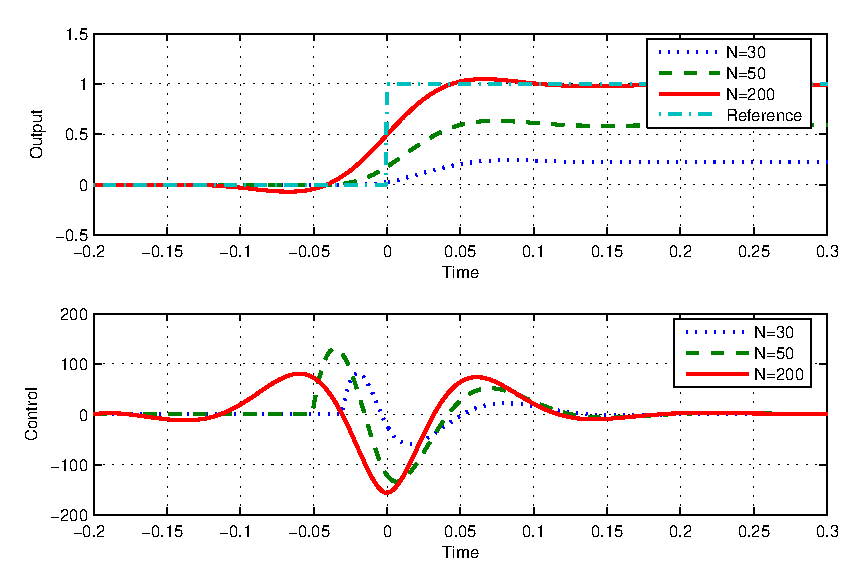
\includegraphics[width=\columnwidth]{./diags/BetterSSwithIncN.eps}
\caption{Closed-loop response of the system described in (\ref{example}) and Figure~\ref{fig:PrevTrackSysFI} with $W_r=1$ and $W_e=1000$.
The plotted output is the signal $z_g$ in Figure~\ref{fig:PrevTrackSysFI}, and shows the relative non-responsiveness of the low-preview-horizon system.
\label{fig:BetterSSWithIncN}}
\end{figure}
%Changes merged to here
\item[Reference weighting introduces stochastic preview.] 
The responses illustrated in Figure \ref{fig:BetterSSWithIncN} are unsatisfactory for preview horizons of less than $N=200$. When short preview horizons are mandated, a low-pass $W_r$ improves low frequency tracking by biasing the controller optimisation towards lower frequencies. It is worth noting, however, that care should be taken in choosing $W_r$.
If, for example, $W_r$ rolls off too quickly, the closed-loop will be poorly tuned for step inputs and can have an oscillatory response, and/or high-amplitude controls. This is because a low-pass $W_r$ has the dual effect of penalising low frequency tracking errors, and also reducing the penalty on high frequency controls -- see (\ref{eqn:DesInsightCL}).
The effect of a low-pass $W_r$ is illustrated in Figure~\ref{fig:WrWithIncreasingPreview}.
\begin{figure}
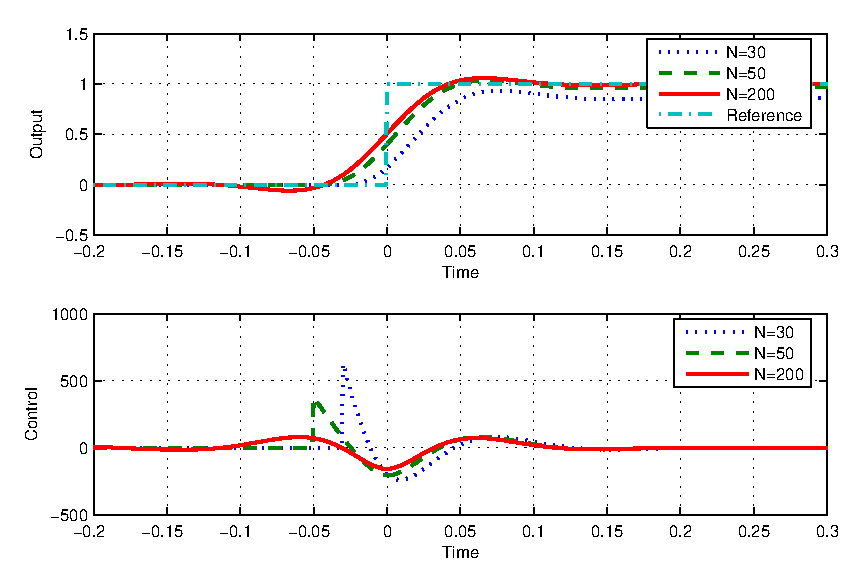
\includegraphics[width=\columnwidth]{./diags/WrWithIncreasingPreview.eps}
\caption{Closed-loop response of the system described in (\ref{example}) and Figure~\ref{fig:PrevTrackSysFI}; the reference weight is given by $W_r=\z/(\z-0.99)$, with $W_e=1000$. The improved step response (of $z_g$) for short preview horizons is clearly visible. Note the high-amplitude control in the $N=30$ case. \label{fig:WrWithIncreasingPreview}}
\end{figure}
\item[Tracking-error filtering.]
Consider the Full Information controller synthesis problem illustrated in Figure~\ref{fig:PrevTrackSysFI} and let $W_e$ be a dynamic
tracking-error filter. A low-pass weight on the tracking error improves the steady-state tracking performance, without needing to change the assumed frequency content of the reference signal (i.e. without changing $W_r$). Even if $W_r=1$,  the inclusion of a low-pass tracking-error filter ($W_e$) ensures that the low-frequency components of $r$ will be tracked accurately, in contrast to Figure~\ref{fig:BetterSSWithIncN}. This is accomplished via feedback based on the states of $W_e$, which is low-pass and so there is no initial `spike' in the control signal -- see Figure \ref{fig:ReducingControlWithIncreasingN}. 
\item[Improving the low-frequency tracking behaviour.]
It appears that there are three alternative ways of improving the low-frequency tracking behaviour, which could be used alone or in combination: (A) use a long preview horizon; (B) add a low-pass reference filter, and (C) introduce a low-pass tracking-error filter. These alternatives are illustrated in Figure~\ref{fig:CompWzWrNormForSimilarResp}. In order to achieve a fair comparison, $W_e$ was scaled so that the resulting closed loops achieved approximately similar rise times. The tracking-error filter achieves good steady-state performance without excessive control, or large control spikes.
However, the introduction of a tracking-error filter tends to introduce additional phase lag, which can have a deleterious effect on the loop's robust stability. In contrast, the feedback part of the controller is independent of $W_r$, which means that a reference filter can be used without jeopardising stability.  
\begin{figure}
\begin{center}
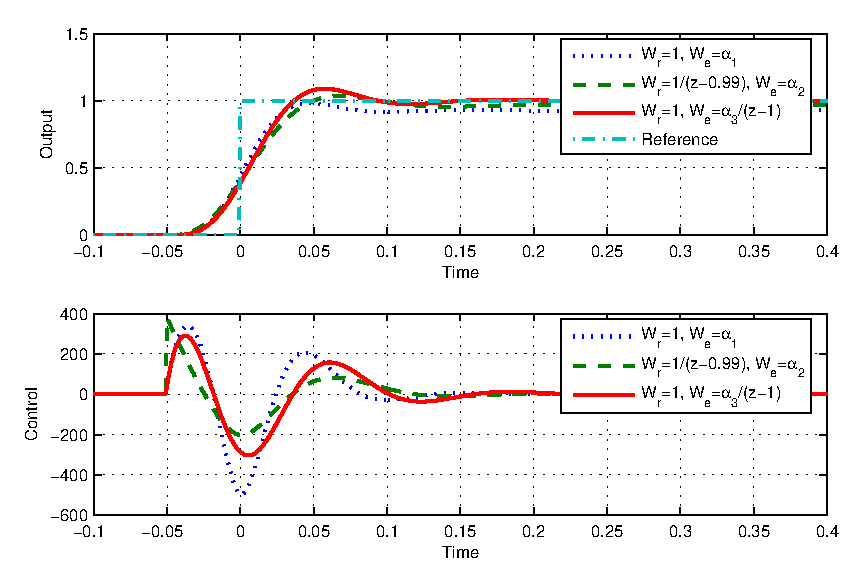
\includegraphics[width=\columnwidth]{./diags/CompWzWrNormForSimilarResp.eps}
\end{center}	
\caption{Closed-loop response of the example system described in (\ref{example}) and Figure~\ref{fig:PrevTrackSysFI}. The preview horizon is fixed at $N=50$ and $\alpha_i$ is used to achieve similar closed-loop rise times. While the closed-loop responses ($z_g$) are similar, the control signals are quite different; especially near the beginning of the preview horizon. \label{fig:CompWzWrNormForSimilarResp}}
\end{figure}
\item[Preview reduces the peak control magnitude.] 
Figure~\ref{fig:ReducingControlWithIncreasingN} illustrates the influence of preview on the control magnitude. In this example, the output response is not strongly influenced by changes in the preview horizon, but the peak control magnitude reduces substantially as the preview horizon increases. This effect can be very useful in application in which control ceilings are a limiting factor, and one wishes to maintain a short rise time.
\begin{figure}
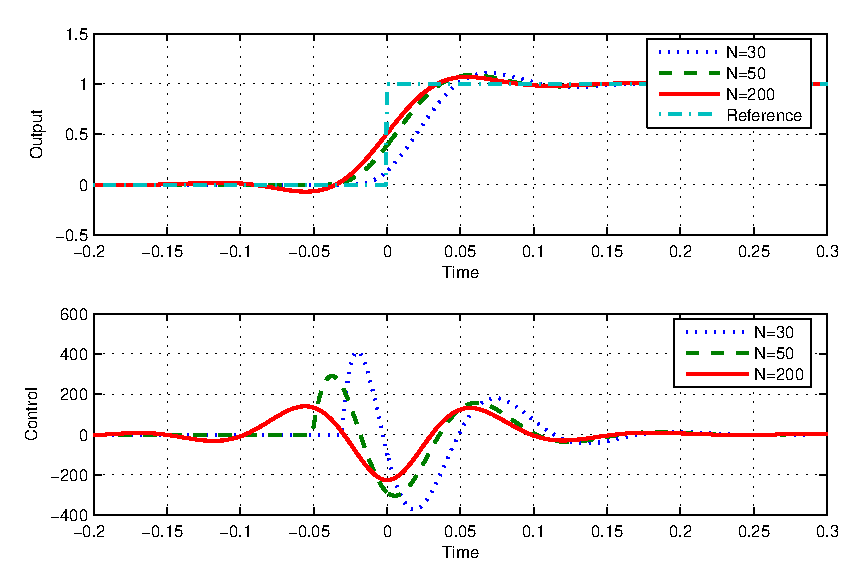
\includegraphics[width=\columnwidth]{./diags/ReducingControlWithIncreasingN.eps}
\caption{Closed-loop response of the example system described in (\ref{example}) and Figure~\ref{fig:PrevTrackSysFI}; the weighting functions are $W_r=1$ and $W_e=100/(1-\z)$. The plotted output is the signal $z_g$ in Figure~\ref{fig:PrevTrackSysFI}, and is relatively insensitive to the preview horizon. The control signal becomes `spread out', and lower in amplitude, as the preview horizon is increased. \label{fig:ReducingControlWithIncreasingN}}
\end{figure}
\item[Preview only improves low frequency tracking performance.] For a low-pass plant, high frequency tracking performance is limited by the prohibitive size of the control action, which is a fundamental feature of the plant and cannot be changed by anticipative action. This effect is illustrated in Figure~\ref{fig:sigmah2}. In this example, preview improves the low-frequency performance by reducing the magnitude of both the tracking error and the control signal. %The price for this improvement appears to be larger control action at higher frequencies
\begin{figure}
\subfloat[Unweighted plant]{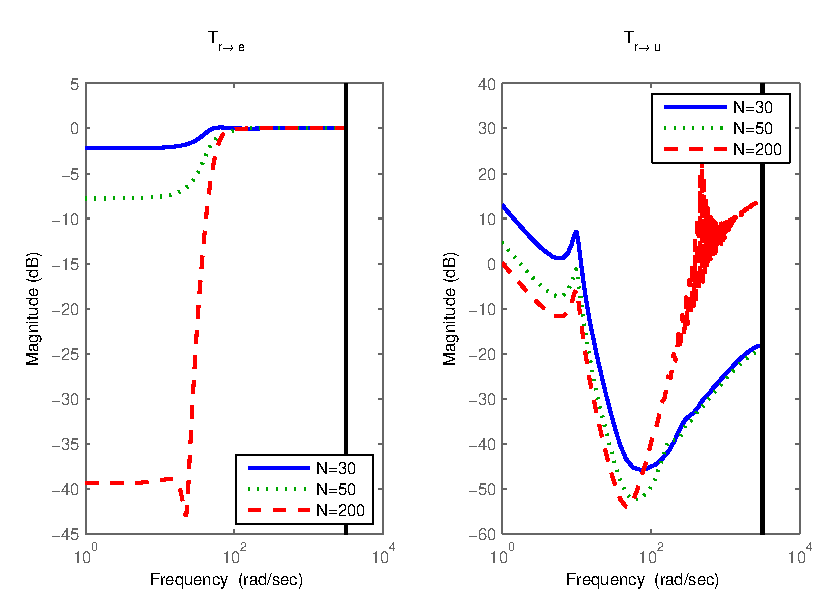
\includegraphics[width=\columnwidth]{./diags/UnweightedSigmaH2.eps}}

\subfloat[$W_e=\frac{1}{\z-1}$]{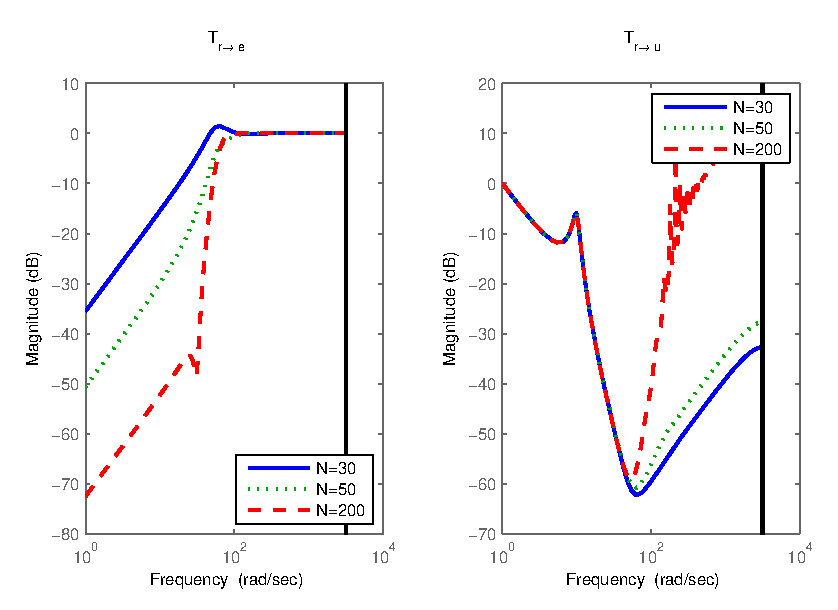
\includegraphics[width=\columnwidth]{./diags/WeightedSigmaH2.eps}}
\caption{Bode plots of the closed-loop transfer functions $T_{r\rightarrow e}$ and $T_{r\rightarrow u}$ which result from application of the $\hinf$-optimal controls.\label{fig:sigmah2} The unweighted plant is considered in (a), and a low-pass $W_e$ is employed in (b).}
\end{figure}
\item[Integral action with output feedback.]
An output-feedback tracking controller with integral action is described by Figure \ref{fig:TrackSysIntegDesign}, which also serves to
illustrate the complexity of problems that may be tackled  using the framework in Figure 1. The integrated error signal must be included in the measurements in order to ensure that the integrator state is detectable. 
Tuning the relative magnitudes of $W_{e1}$ and $W_{e2}$ is akin to adjusting the gains in a PI controller. The ability to adjust the integral gain is useful, because too much integral action can be detrimental to stability and/or the transient response. In fact a `derivative' signal could also be added, thus completing the PID analogy and facilitating tuning of the preview controller. 

Previous approaches to the addition of integral action have done so in an \ac{LQG} setting through the use of the differentiated control signal in the cost function \citep[e.g. ][]{Tomizuka_1979_IntegralPreviewFI,Katayama_1987_PreviewAndIntegral,Tomi_1980_FFPrev}. Such an approach does not allow one to adjust the strength of the integral action, which could lead to difficulty in satisfying stability/performance requirements. 


\begin{figure}
\begin{center}
\stdcontrolfrags
\psfrag{W_e1}{$W_{e1}$}
\psfrag{W_e2}{$W_{e2}$}
\psfrag{W_n}{$W_{n}$}
\psfrag{z1}{$z_1$}
\psfrag{z2}{$z_2$}
\psfrag{z3}{$z_3$}
\psfrag{y1}{$y_1$}
\psfrag{y2}{$y_2$}
\psfrag{I1/(z-1)}{$I\frac{1}{\z-1}$}
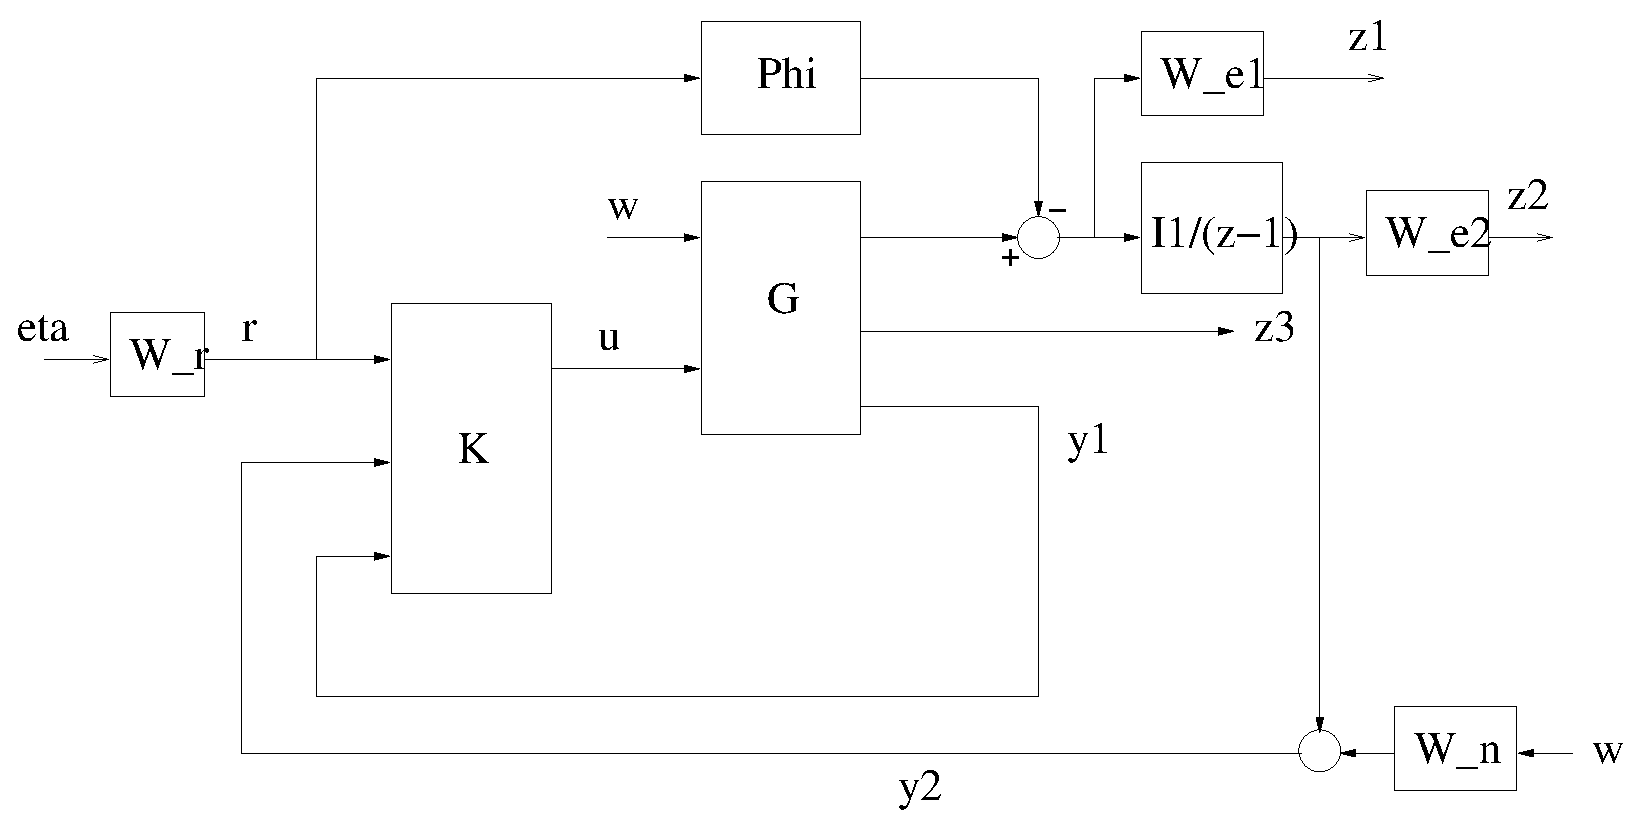
\includegraphics[width=12cm]{./diags/TrackSysInteg.eps}
\end{center}
\caption{Preview tracking with integral action. The signal $z=\left[z_1'\,\,z_2'\,\,z_3'\right]'$ is the output of the closed-loop transfer function
whose 2-norm is to be minimised; $y=\left[y_1'\,\,y_2'\right]'$ is the measurement signal. The transfer functions $W_{e1}$, $W_{e2}$ and $W_n$ are shaping filters. Other notation follows that of Figure \ref{fig:DistRejSys}. \label{fig:TrackSysIntegDesign}}
\end{figure}

\end{description}
 


 





